
\chapter{活动概念抽取}
\section{数据来源}
本文的工作基于新浪微博的数据。我们随机选取了100个用户作为种子,并获取他们的关注者和关注他们的人。

\section{分词及词性标注}
中文分词一直自然语言处理中很基础的一步,常用的中文分词工具,如哈工大的LTP,中科院的ICTCLAS, Stanford Parser,实际应用中都难以做到非常高的准确度,尤其是在微博这种格式自由,用语不规范的文本中。综合比较各个工具的速度、精度后,我选择了ICTCLAS作为分词工具。

\section{短语抽取}
一项活动通常以一个动词(如睡觉,游泳,跑步)或者一个动词和一个名词对象组成的动宾短语(如吃午饭,去学校,打篮球)表示。为了挖掘出微博中表达的活动,我们需要将频繁出现的短语抽取出来,以待进一步处理。

最简单的方法是,遍历语料,统计所有动词短语(包括单独的动词,相邻的动词和名词)的频度,按照词频保留TopK个。这样做有两个问题
\begin{itemize}
\item 受停用词影响很大。汉语中的一些停用词,如``是'', 常被归为动词。另一些虽然不是传统意义上的停用词,一般不做为一个动作,而是副词,如``完''”,``过'' 但经常出现在动词短语中,如``做完作业'',``吃过午饭''等,干扰短语的识别。这些词的数量有限,可以简单总结,扩充已有的停用词典,预先进行过滤。
\item 目标短语在文本中可能不是连续的。除了上面举过的例子之外,动词和名词之间可能包含一些更复杂的语言成分,如``买了一件衣服'', ``参加学校举办的比赛''。由于当前的目标是抽取常见的动词短语,而并不关注单句话的精确解析,因此可以忽略过于复杂的情况,将一些常见情形总结成规则进行匹配。
\item 倾向于选取包含高频词的短语。多次同时在一起的动词、名词组合不一定是一个合法的短语,而仅仅基于词频选取短语,会倾向于包含高频词的词组。如果一个词出现次数非常高,它随机地和其他词语一起出现的次数也相应增加,导致抽取结果中包含很多噪声。为了解决这一问题,我们衡量两个词$<w_i, w_j>$构成词组概率为
$\frac{P(<w_i, w_j>)}{P(w_i)P(w_j)}$, 同时限定$n_{<w_i,w_j>} > min_support$.最后,我们按照$ln(n_{<w_i, w_j>}) + \lambda\frac{P(<w_i, w_j>)}{P(w_i)P(w_j)}$递减选取了160,000条候选短语。
\end{itemize}

\section{获取语义向量表示}

\subsection{目标与相关背景}
接下来,我们需要对得到的短语,包括unigrams和bigrams进行分类,以识别哪些短语表示一个活动。对于bigrams,它由一个动词和名词组成,一种显而易见的想法是,包含特定动词的短语,比如( 吃, ), (去, ) 更有可能是一个Activity,如果我们进行足够多的标注,就能进行有效的分类.即,每个词对应一个向量,词$w_i$对应的向量中,只有对应词序号的分量为1,即$(0_1, 0_2, ... , 1_i, ... , 0_n)$, 在计算语言学中称为One-hot Representation. 把它作为特征训练分类器.但这样做有很大的问题。直觉上,假如两个词的语义相似,那么他们的类标更有可能相同;而One-hot representation完全没有考虑词之间的语义相关性,我们能进行的标注量有限,反映到结果上就是精度尚可,但召回率非常低。我们需要找到一种有效的方式衡量两个词的语义相似性。如果能把词表示成一个K维语义空间中的一个向量,K远远小于不同词的总数,用向量的余弦相似度或者欧氏距离来衡量相似性,是最理想的,这是词的Distributed Representation,它由Hinton在1986年提出\cite{hinton1986learning}。

\subsection{话题模型}
以LDA\cite{blei2003latent}为代表的话题模型可以作为一种获得单词向量表示的方法。TODO

\subsection{n-gram 语言模型}
要对语义进行建模,容易想到的思路是,假如两个词经常出现的上下文相似,那么它们的语义可能也是相似的,这是自然语言处理中了统计语言模型的基础。一个语言模型是语言基本单位(如句子)的生成模型,用各个单词出现的条件概率来表示,即
\[
p(sentence) = \prod\limits_t {p({w_t}|Context_t)}
\]
Context的选取不同,语言模型也随之变化,其中n-gram语言模型是其中常用的一种。它对语言的生成做了n-1阶Markov假设,一个词的出现概率仅和前n-1个词相关,即
\begin{align*}
Context_t = & w_{t-n+1}^{t-1} \\
		= & (w_{t-n+1}, w_{t-n+2}, \ldots, w_{t-1}) \\
p(sentence) = & \prod\limits_t {p({w_t}|w_{t-n+1}^{t-1})}
\end{align*}

n-gram语言模型的问题是,由于语料的限制,高阶的语言模型受制于数据的稀疏性,无法建模更远的关系,一般使用tri-gram。随着互联网带来的海量数据以及计算能力的提升,更高阶的语言模型成为可能,Google曾经公开了5-gram的语言模型,但体积非常大,对我们的应用来说不切实际的。

其次,n-gram对语义相似度建模的能力有限。它仅考虑词在给定上下文出现的概率,但对上下文的相似性没有考虑。比如,``房间里趴着一只狗''和``卧室里趴着一只猫'',对``猫''和``狗''建模时,n-gram模型没有考虑``房间''和``卧室''的相似性,而它们的相似性是可以根据其他文本得到的。我们需要找到一种可以将上下文相似性一并考虑的方法模型。

\subsection{神经网络语言模型(NNLM)}
换个角度思考,我们要求的是$p({w_t}|w_{t-n+1}^{t-1})$, 实际可以看做是一个函数$f(w_{t-n+1}, w_{t-n+2}, \ldots, w_{t-1}, w_t)$. Hornik等人证明了,带有一个隐含层的多层前馈神经网络,可以近似$R^n$上任意连续函数(universal approximation theorem\cite{hornik1991approximation}). 因此,我们也能用神经网络来逼近$f()$. 我们把$w_{t-n+1}, w_{t-n+2}, \ldots, w_{t-1}$的One-hot Representation作为输入,希望输出$output_i=P(w_t=i|w_{t-n+1}, w_{t-n+2}, \ldots, w_{t-1})$, 这样就是n-gram语言模型的神经网络近似。如果我们把输入换成每个词对应的K维向量表示,那么上下文的相似性可以自然体现在向量的相似性中,这个模型就是神经网络语言模型(NNLM)\cite{bengio2006neural} \cite{mikolov2013efficient}。与一般神经网络不同的是,它的输入,即每个词的向量表示,是未知的,需要和模型参数一同优化。

\subsection{使用前馈神经网络训练NNLM}

\subsection{案例研究}
我们在1300万条新浪微博上训练了NNLM,并对得到的向量做一些案例研究,以检验模型的有效性。

通过神经网络语言模型训练得到的词向量,的确反映了语义层面上的特征,可以用余弦相似度衡量两个词语义上的相关性。我们给出一个活动,找出和其最相似的10个词组,衡量其相关性:

\begin{table}[h]
\centering
\begin{subtable}{0.3\textwidth}
     \begin{tabular}{|l|c|} 
	\hline
	{\heiti 短语} & {\heiti 相似度} \\
	\hline
	打\_篮球 & - \\
	\hline
	打球 & 0.800 \\
	\hline
	踢\_足球 & 0.790 \\
	\hline
	打\_网球 & 0.789 \\
	\hline
	打\_羽毛球 & 0.797 \\
	\hline
	踢球 & 0.727 \\
	\hline
	踢\_球 & 0.697 \\
	\hline
	练\_球 & 0.686  \\
	\hline
	游泳 & 0.667 \\
	\hline
	排球 & 0.651 \\
	\hline
	打\_排球 & 0.649 \\
	\hline
	\end{tabular}
\end{subtable}
\hspace{1em}
\begin{subtable}{0.3\textwidth}
	\begin{tabular}{|l|c|} 
	\hline
	{\heiti 短语} & {\heiti 相似度} \\
	\hline
	打扫 & - \\
	\hline
	打扫\_卫生 & 0.805 \\
	\hline
	收拾 & 0.757 \\
	\hline
	洗\_衣服 & 0.747 \\
	\hline
	家里\_打扫 & 0.699 \\
	\hline
	收拾\_屋子 & 0.693 \\
	\hline
	搞\_卫生 & 0.666 \\
	\hline
	捣鼓 & 0.659 \\
	\hline
	打扫\_打扫 & 0.659 \\
	\hline
	洗\_床单 & 0.654 \\
	\hline
	拖\_地板 & 0.652 \\
	\hline
	\end{tabular}
\end{subtable}

\begin{subtable}{0.3\textwidth}
	\begin{tabular}{|l|c|} 
	\hline
	{\heiti 短语} & {\heiti 相似度} \\
	\hline
	吃\_晚饭 & - \\
	\hline
	吃\_午饭 & 0.920 \\
	\hline
	晚饭 & 0.844 \\
	\hline
	吃\_中饭 & 0.831 \\
	\hline
	吃饭 & 0.816 \\
	\hline
	吃\_夜宵 & 0.795 \\
	\hline
	吃\_早饭 & 0.780 \\
	\hline
	午饭 & 0.777 \\
	\hline
	出去\_觅食 & 0.755 \\
	\hline
	中午\_饭 & 0.746 \\
	\hline
	喝\_早茶 & 0.736 \\
	\hline
	\end{tabular}
\end{subtable}
\hspace{1em}
\begin{subtable}{0.3\textwidth}
	\begin{tabular}{|l|c|} 
	\hline
	{\heiti 短语} & {\heiti 相似度} \\
	\hline
	下班 & - \\
	\hline
	上班 & 0.751 \\
	\hline
	回家 & 0.748 \\
	\hline
	下班\_回家 & 0.730 \\
	\hline
	坐\_班车 & 0.716 \\
	\hline
	提早\_下班 & 0.706 \\
	\hline
	回到\_家 & 0.705 \\
	\hline
	十一点\_半 & 0.705 \\
	\hline
	五点\_下班 & 0.703 \\
	\hline
	吃\_晚饭 & 0.701 \\
	\hline
	收工 & 0.698 \\
	\hline
	\end{tabular}
\end{subtable}

\caption{相似度实例}
\end{table}


并且词向量具有可加性.例如, 可以用向量加法来表达语义关系的组合:
\begin{align*}
	v(\text{济南}) - v(\text{山东}) + v(\text{浙江}) \approx & v(\text{杭州}) \\
	v(\text{北京}) - v(\text{中国}) + v(\text{法国}) \approx & v(\text{巴黎}) \\
\end{align*}
这里的约等于号表示,在所有的词中,约等号右边的词与左边运算的结果余弦相似度最大.这两个式子的含义是,杭州对浙江的关系,与济南对山东的关系相似(都是省会); 东京对日本的关系,与北京对中国的关系相似(都是首都).

再比如
\begin{align*}
	v(\text{喝}) - v(\text{渴}) + v(\text{饿}) \approx & v(\text{吃}) \\
	v(\text{校长}) - v(\text{学校}) + v(\text{公司}) \approx & v(\text{总裁}) \\
	v(\text{胡锦涛}) - v(\text{中国}) + v(\text{日本}) \approx & v(\text{首相}) \\
\end{align*}

这些式子都有很明确自然的语义关系.
当然,这种语义组合的关系并不是总能成立.

\section{最优化标注集}

下一步,我们对抽取出的候选集进行分类。每个短语可以看做K维语义向量空间中的一个向量,更确切来说,由于每个向量的模长均为1,它们分布在一个K维超球面上.并且由于语义的复杂性,正例(表示活动的短语)和负例(无关短语)是线性不可分的。对于模型的选择,我们主要考虑使用现有的可处理非线性情形的机器学习模型,如K近邻,支持向量机SVM,决策树等等,逻辑回归Logistic Regression等线性模型也进行测试。

分类器训练通常需要对训练样本进行标注,人工识别每个短语的类别,以确定模型参数,训练样本一般是从待分类数据中随机抽样得到。由于语义空间很大,待分类的数据也比较多,而我使用随机抽样得到的训练样本直接训练一个SVM分类器,精度可以达到76\%, 但是召回率非常低,只有43\%。更多的标注可以改善召回率低的情况,但是由于数据量很大,大量标注是很耗时的。由于数据分布的特殊性,我希望设计一种有原则的(Principled)训练样本抽取方法,在标注数据量一定的情况下,能够尽可能提高训练的效果。假设标注集为$L$,我们需要恰当定义其效用函数$Q(L)$以判断它的有效性,并且在一定约束条件下,找出最优的$L$,也就是

\[
    L^* = \arg\max_{L,|L| = M} Q(L)
\]

直觉上考虑,标注一个训练样本后,和此训练样本相似的样本,我们有较高的置信度将其正确分类。以K近邻分类器为例,对于每个未知样本,寻找训练集中和其距离最近的K个样本,由这K个近邻投票确定此样本的类标。但在我们的问题中,样本间的相似性$sim(v_i, v_j)$使用向量的余弦相似度来表示$<v_i, v_j$,据此可以定义一个样本$v$和集合$S$的相似性。

\begin{definition}
\[
    sim(v, S) = sim(v, u),|\{ {v_j}|sim({v_j},v) \ge sim(u,v)\} | = K
\]
\end{definition}

即,集合中和$v$第K个和其最相似的元素的相似度。设全部样例的集合为$U$, 标注集为$L$, 我们的效用函数可以定义成
\[
    Q(L) = \mathop {\min }\limits_{{v_i}} si{m_K}({v_i},L)
\]

目标是找到最优的标注集$L^*$。我们的问题可以形式定义为:
\begin{problem}\label{label:opt_problem}
给定集合$U$, 对任意元素$v_i, v_j \in U$, 有相似度度量$sim(v_i,v_j)$. 元素与集合相似度$sim_K(v, S)$如前定义。我们要求
\[
        {L^*} = \mathop {\arg \max }\limits_L Q(L),|L| = M, L \subseteq U
\]
\end{problem}

\ref{label:opt_problem}是一个组合优化问题,类似于k-center问题,但是我们用的相似度度量不满足三角不等式,现有算法无法直接应用。通常来说,这类问题是NP-Hard的,下面我们将集合覆盖问题可以归约到此问题来证明其NP-Hardness。集合覆盖问题的判定版本是Richard Karp在1971年提出的21个NP完全问题之一。问题定义为:

\begin{problem}[集合覆盖]
给定全集$U$,一族子集$S=\{S_i\}, \cup {S_i} = U$,以及整数$M$,判定是否存在覆盖$[C \subseteq S,|C|=M$,使得$\cup \{ {S_i}|{S_i} \in C\}  = U$
\end{problem}

显然,如果任意K,我们能在多项式时间解决,K=1也是可以的。当K=1时,此问题的判定版本是,给定阈值$\theta$,问是否存在大小为$M$的集合$L$,使得
\[
    \theta  \le \mathop {\min }\limits_{{v_i} \in U} \mathop {\max }\limits_{{v_j} \in L} \{ sim({v_i},{v_j})\} 
\]
如果能证明K=1时判定问题的NP完全性,那么原问题的NP-Hardness就得证。

\begin{proof}
对于集合覆盖问题,如果存在一个元素$v\in U$不在任何一个$S_i$中,那么覆盖显然是不存在的,因此下面仅考虑每个元素都至少被一个元素覆盖的情况。

设$|U| = N, |S| = P$, 我们构造一个包含$N+P$个结点的图$G=(V,E)$。其中,集合$U$中的每个元素$v_i, 1 \le i \le N $ 都是$G$中的一个结点,称为元素结点(element nodes),此外,对每个$S_i \in S$, 创建新节点$v_{i+N}, 1 \le i \le P$, 称作集合结点(set nodes)。$E={(v_i, v_{j+N}) | v_i \in S_j, 1\le i \le N, 1\le j \le P} \cup {(v_i+N, v_j+N) | 1 \le i,j \le P}$. 也就是说,每个集合都和它包含的元素连边,集合之间两两连边。所有边赋权为$\theta$,不存在边的赋权负无穷。如下图所示。
\begin{figure}[htbp]
\centering
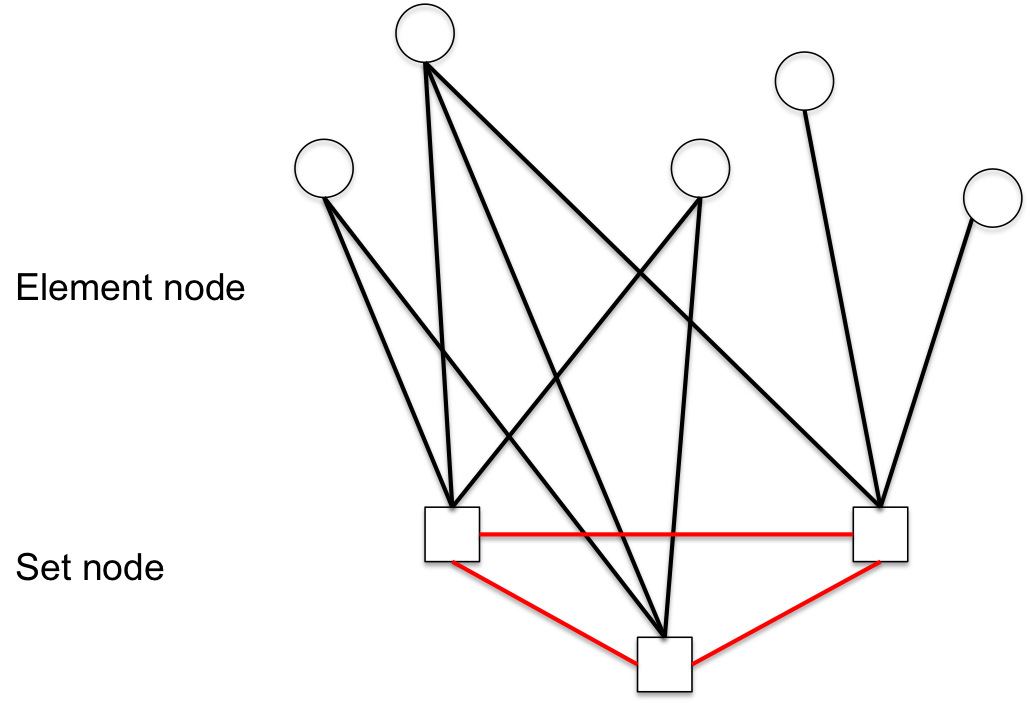
\includegraphics[width=0.6\textwidth]{./setcover.png}
\caption{集合覆盖-距离}
\label{fig:setcover}
\end{figure}


假如我们能在多项式时间内求解原问题。如果存在$L^*$,则取$L^*$对应集合的结点(如果对应元素,替换成任意一个包含它的集合),这样我们就找到了$U$的一个覆盖。如果$L^*$不存在,则集合覆盖也不存在。因此,我们要求解的判定问题是一个NP完全问题。故优化问题是一个NP-Hard问题。不存在已知的多项式时间解。
\end{proof}


\subsection{子模性及近似求解}
前文已经证明最优化$Q(L)$是一个NP-Hard问题,但是下面我们将证明其单调性和子模性,并据此得到一个贪心算法(greedy algorithm), 在多项式时间内得到近似解$Q(L')$, 并且保证
\[
	Q(L^*) \ge (1-\frac{1}{e}) Q(L')
\]

\begin{definition}[子模函数]
从幂集$2^\Omega \to R$的一个函数$f$称为子模函数(submodular function),如果对任意$X,Y \subseteq \Omega, X \subseteq Y$,$\forall x \notin Y$, 有$f(X \cup \{x\} ) - f(X) \geq f(Y \cup \{x\} ) - f(Y)$.
\end{definition}

下面我们分别证明$Q(L)$的单调性和子模性。
\begin{proof}[单调性]
令集合$Y=X\cup{x}$。对任意元素$y \in U - X$, 设$sim_K(y, X) = sim_K(y, t), t \in X]$,
那么,
\[
	|\{ {v_j}|sim({v_j},v) \ge sim(y, t), v_j \in X \} | = K	
\]
由于$X \subset Y$,故有
\[
	|\{ {v_j}|sim({v_j},v) \ge sim(y, t), v_j \in Y \} | \ge K	
\]
从而, $sim_K(y, Y) \ge sim_K(y, X)$。由$y$的任意性,得到
\[
	Q(Y) \ge Q(X)
\]
单调性证完。
\end{proof}

\begin{proof}[子模性]
设集合$X \subset Y$, 对任意$x \in U - Y$, 设$X' = X\cup{x}, Y' = Y\cup{y}$。
对任意$y \in U$, 由单调性有
\[
	sim(y, Y') \ge sim(y, X') \ge sim(y, X) \\
	sim(y, Y') \ge sim(y, Y) \ge sim(y, X) 
\]

对于新加入的元素$x$, 有
\begin{align*}
	sim(y, X') = & \max\{ sim(y, x), sim(y,X) \} \\
	sim(y, Y') = & \max\{ sim(y, x), sim(y,Y) \} \\
\end{align*}

于是
\begin{align*}
	sim(y, Y') - sim(y, Y) = & \max \{ sim(y, x) - sim(y, Y), 0\} \\
						\le & \max \{ sim(y, x) - sim(y, X), 0 \} \\
						= & \max \{ sim(y, x), sim(y, X) \} - sim(y, X) \\
						= & sim(y, X') - sim(y, X)						
\end{align*}
由$y$的任意性,子模性得证。
\end{proof}

\begin{theorem}
对于一个单调增的子模函数$Q$,从空集$L_0$开始,使用贪心策略进行迭代,即第$k$次迭代选取元素$v_k$,使得
\[
	v_k = \mathop {\arg \max }\limits_{v_k \notin L_{k-1} } Q(L_{k-1}\cup \{v_k\}) 
\]
\[
	L_k = L_{k-1} \cup \{ v_k \} 
\]
那么$K$次迭代之后, 对任意$L, |L| \le K$,有
\[
	Q(L_k) \ge (1-\frac{1}{e}) Q(L'),
\]
\end{theorem}

这直接给我们了一个保证下界的贪心算法。
\begin{algorithm}
  \caption{maximize Q(L)}
  \KwIn{Unisersal set $U$, target size $K$ and similarity measure $sim()$}
  \KwOut{${L^*} = \mathop {\arg \max }\limits_{L,|L| = K, L \subseteq U} Q(L)$ }
  $L_0 = \emptyset$\;
  \For{$k=1;k \le K;k += 1$}
  {

  }
  return $con(r_i)$\;
\end{algorithm}

\section{模型选择}
我们的标注集选择和KNN有密切的联系,KNN在我们的数据中可能表现更好,但是我们也会尝试其他的分类模型,如支持向量机,随机森林等。

\section{实验结果与错误分析}
为了检验我们标注和分类的效果,我们从短语候选集中随机抽取了5000个短语作为Ground Truth进行测试。

图\ref{fig:testing_vs_random}是我们分别使用随机抽样(Random)和最大化$Q(L)$(MaxSim)的方法选取500、1000、2000个标注样本时,5-NN分类器在测试集上的表现。对于随机抽样,我们进行5次试验取平均值,并在图中标注了最大和最小值。

\begin{figure}[h!]
  \centering
  \begin{subfigure}{0.4\textwidth}
    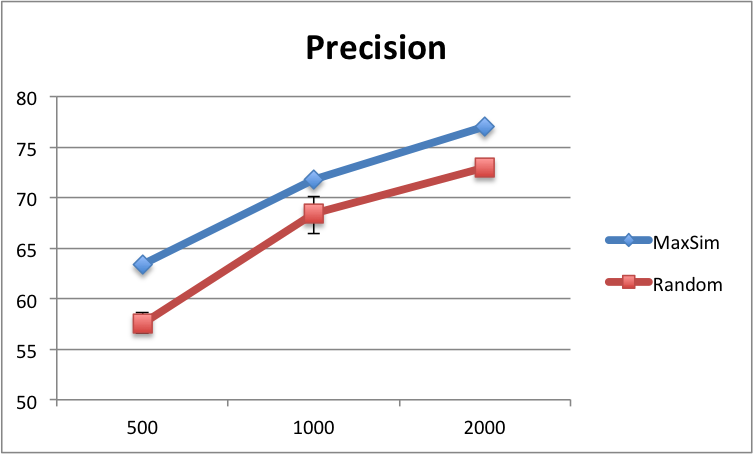
\includegraphics[width=\textwidth]{label_precision.png}
    \caption{Precision}
  \end{subfigure}
  \hspace{2em}%
  \begin{subfigure}{0.4\textwidth}
    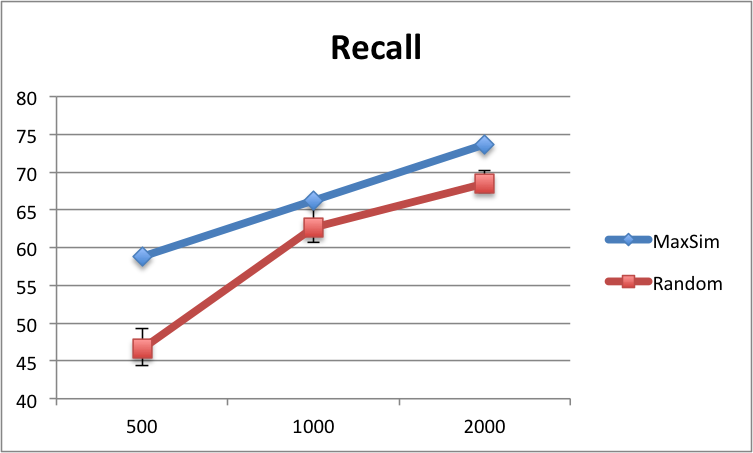
\includegraphics[width=\textwidth]{label_recall.png}
    \caption{Recall}
  \end{subfigure}
  \hspace{2em}
  \begin{subfigure}{0.4\textwidth}
  	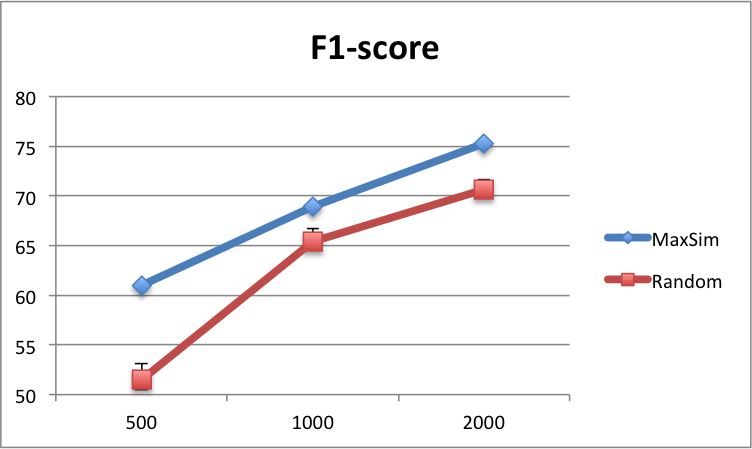
\includegraphics[width=\textwidth]{label_f1.png}
  	\caption{F1-score}
  \end{subfigure}
  \caption{实验结果}
  \label{fig:testing_vs_random}
\end{figure}
从图\ref{fig:testing_vs_random}中可以看出,我们提出了训练集选取方案,在Recall和Precision方面,都稳定的高于随机随机抽样,尤其是在标注量较小时,MaxSim选取的标注集在Recall方面的优势更加明显。

同时我们测试了其他分类模型在两种标注集选取方法下的性能。

可以看出除了KNN以外,SVM,随机森林等分类器在MaxSim上的性能都超过了随机方法。同时,SVM和KNN的总体表现(F1-score)上相差不多,Precision较高而Recall较低,在实际系统中,我们希望提供更加精确的结果,因此,我们最终采用SVM作为分类模型。

\section{错误分析和性能优化}
我对分类错误的样本


